% add. options: [seceqn,secthm,crcready,onecolumn]
\documentclass[sw]{iosart2x}

%\usepackage{dcolumn}
%\usepackage{endnotes}
\usepackage{booktabs}
\usepackage{tabulary}
\usepackage{csquotes}
\usepackage{siunitx}
%\usepackage{graphicx}
\usepackage{todonotes}
%\usepackage{natbib} % does not seem to work with ios 1
\renewcommand{\citet}{\cite}% citet is not defined without natbib
\renewcommand{\citep}{\cite}% citep is not defined without natbib
\setlength{\marginparwidth}{2.1cm}% enough space for todonotes
\usepackage{listings}
\usepackage{aurl}
\daurl{bb}{http://www.snik.eu/ontology/bb/}
\daurl{meta}{http://www.snik.eu/ontology/meta/}
\lstset{language=SPARQL,breaklines=true}
\usepackage{cleveref}
\newcommand{\snikversion}{1.0}
\newcommand{\sniktriples}{72046}
\newcommand{\snikclasses}{2655}
\newcommand{\snikproperties}{339}
\newcommand{\sniklinks}{581}
%%%%%%%%%%% End of definitions

\pubyear{2020}
\volume{0}
\firstpage{1}
\lastpage{1}

\begin{document}

\begin{frontmatter}

%\pretitle{}
\title{SNIK: Textbook Knowledge on Hospital Information Management as Linked Data}
%\runningtitle{The SNIK Ontology of Hospital Information Management}
%\subtitle{}

% Two or more authors:
\author[A]{\inits {K.}\fnms{Konrad} \snm{Höffner}\ead[label=e1]{konrad.hoeffner@imise.uni-leipzig.de}%
\thanks{Corresponding author. \printead{e1}.}},
\author[A]{\fnms{Franziska} \snm{Jahn}\ead[label=e2]{franziska.jahn@imise.uni-leipzig.de}},
\author[A]{\fnms{Birgit} \snm{Schneider}\ead[label=e3]{birgit.schneider@imise.uni-leipzig.de}},
%\author[A]{\fnms{Anna} \snm{Lörke}\ead[label=e4]{anna.loerke@imise.uni-leipzig.de}},
\author[A]{\fnms{Thomas} \snm{Pause}\ead[label=e5]{thomas.pause@imise.uni-leipzig.de}},
\author[A]{\fnms{Alfred} \snm{Winter}\ead[label=e6]{alfred.winter@imise.uni-leipzig.de}}
%\runauthor{K. Höffner et al.}
\address[A]{Institute for Medical Informatics, Statistics and Epidemiology (IMISE),
\orgname{University of Leipzig}, \cny{Germany}\printead[presep={\\}]{e1,e2,e3,e5,e6}}
%Medical Informatics, Management of Health Information Systemsi
%Härtelstraße 16--18, D-04107 Leipzig

\begin{abstract}
%Textbooks contain abstract knowledge about a domain.
Textbooks about information management in hospitals describe the planning, monitoring and directing of a hospital's information system.
SNIK consists of the manually transformed content of three such textbooks as Linked Open Data.
The data model describes information management functions, roles executing these functions and the information used or updated by these functions.
%SNIK provides applications that are used to teach students internationally.
%and the result of applying the data model to three textbooks, an interview and a standard.
%To compare, 
%, making it a natural fit for RDF, RDFS and OWL.
%As the domain is large and highly relevant to students of Medical Informatics, modelling the knowledge is not only possible but also very useful.
We publish the result over several different interfaces that are useful for researchers, information system administrators or students, depending on their objectives and their capabilities.
\end{abstract}

\begin{keyword}
\kwd{information management, information systems, hospital information management}
\end{keyword}

\end{frontmatter}

\begin{table}
\caption{}
\label{tab:namespaces}
\begin{tabular}{ll}
\toprule
\textbf{x}	&\textbf{y}\\
\midrule
\bottomrule
\end{tabular}
\end{table}

\section{Introduction}
A health information system (HIS) is the socio-technical subsystem of a care delivery organization~\citep{bb}.
This includes its different application systems, computers, and network components as well as their users.
A HIS processes data, information, and knowledge and its management involves planning, monitoring and directing of those activities.
Due to the complexity and the unique conditions in health care, HIS management is an challenging task.
There are many different frameworks, textbooks and articles describing the scope of HIS management from the perspective of medical informatics.
%However, the disciplines of business informatics and information systems (IS) provide an even broader view on information systems and their management.
%A structured representation of the different perspectives leads to a holistic view on HIS management and helps help researchers and students connect their existing knowledge with further knowledge from other sources during research and learning.
In order to integrate different knowledge sources and to provide the knowledge in a structured, machine-readable data format, we extracted knowledge about HIS management from three textbooks~\citep{bb,ob,he} and other sources.
The combination of this knowledge~\citep{semantischesnetz,domaene,approachtosupport} results in SNIK, the Semantic Network of Information Management in Hospitals (\enquote{Krankenhaus} in German).

In order to encourage and enable other researchers, students and health informatics professionals to use available knowledge of HIS management, We introduce different user interfaces to the SNIK ontology and discuss their suitability for different use cases of the target audiences.
%We discuss advantages and disadvantages of the interfaces and give recommendations on which ones present the best compromise for different use cases and target audiences.
%We conclude with plans for future work on interlinking and visualization.

%As the domain is large and highly relevant to students of Medical Informatics, modelling the knowledge is not only possible but also very useful.
Medical informatics students, who are trained for executive positions in information management departments of healthcare institutions, such as hospitals, need a clear terminology of their domain.
Due to different frameworks and textbooks dealing with information management in healthcare, modelling the knowledge unravels the links between the different views on information management.
These are only implicitly known or not known at all by experts in the field.

We present a common data model for the domain and the result of applying the data model to three textbooks.
We publish the result over several interfaces that are useful for researchers, practitioners and students, depending on their objectives and their Semantic Web skills.

Publishing textbook knowledge as Linked Data enables different ways of teaching.
%The data is continously revised: users constantly report wrong or missing data in the visualization, which is then corrected, respectively revised, by the researchers of the project.


\section{Data Model}
In order to specify, which information should be extracted from the books and to facilitate comparisons, we use a common data model.
Because processed textbooks contain abstract knowledge instead of information about any specific hospital, all concepts are modelled as classes.
We thus call our data model the \enquote{meta model}, as it is an ontology.
meta model in accordance with its definition in the domain as a shared modelling language~\citep[p.~8]{ob}.
The meta model (see \cref{fig:metamodel}) provides a common vocabulary for the domain of HIS management and thus defines, which superclasses and property can be used.
SNIK version \snikversion{} comprises five subontologies that are built upon the meta model, see Table 1.
At the head of the class hierarchy is the \enquote{Top} class, which has exactly three disjunctive subclasses.
Following the meta model, each class has to be a subclass of exactly one of them.
The correct superclass of a new concept can be found by answering the question: Who (\enquote{Role}) does what (\enquote{Function}) and which information (\enquote{EntityType}) is needed? If a concept is neither of them, it cannot be modeled using the meta model.
As the subclass relation is transitive, a new class can be placed further down the hierarchy and it can still be inferred, whether it is a Function, Role or EntityType (see Figure 3).
Besides the subclass relationship, two classes can be connected with relations provided by the meta model.
The generic \enquote{is associated with} relationship carries little information.
For example, a role and a function can be connected as \enquote{is involved in} \enquote{is responsible for} and \enquote{approves}.
Relations that are neither of them can either be modeled by using the generic \enquote{is associated with} relation or by creating and using a new sub relation of \enquote{is associated with}

As a concession to practicality, we express each geleral rule extracted from a textbook as a single triple using classes as subject and object, and a property of the meta model.
For example, the rule "the CEO is involved in project reviews" is modelled as \enquote{\texttt{:Ceo} \aurl{meta}{isInvolvedIn} \texttt{:ProjectReview}.}, where \texttt{:Ceo} is a subclass of \aurl{meta}{Role} and \aurl{meta}{ProjectReview} is a subclass of \aurl{meta}{Function}.
While an OWL restrictions using \aurl{owl}{someValuesFrom} and \aurl{owl}{allValuesFrom} would be technically correct, the knowledge is not expressed that specifically in the textbooks.
Additionally, encoding each fact as a single triple facilitates tool support and prevents inconsistencies through non-atomic changes.

\paragraph{}

%\section{Data Quality}
%- extractors not always same people who wrote book/part of book
%- mistake when extracting
%- reasoning does not work (test)
%\begin{itemize}
%\item Multiple Subtops
%\item Inconsistent Subtop with Subclass
%\item SKOS Link to Different Subtop
%\item Subclass Cycles
%\item Missing superclass
%\item Undefined Objects
%\item Domain Violation
%\item Range Violation
%\item Class URL Naming Convention Violations
%\item Property URL Naming Convention Violations
%\item Missing Definition
%\item Literals with Semicolons
%\item Classes with too many subclasses
%\item No Restriction
%\item Non-HTTP URI
%\item OWL 2 DL: Undefined Properties
%\item OWL 2 DL: Multiply Defined Properties
%\item OWL 2 DL: Class Typing Constraints
%\end{itemize}
%-> use SHAPE/SHACL ?

\section{Unsorted}


\begin{table}
\caption{Access Options and Details}
\label{tab:access}
\begin{tabulary}{\columnwidth}{lL}
\toprule
URL		&\url{http://www.snik.eu/ontology}\\
Version		&\snikversion{}\\
License		&CC BY-NC-SA 4.0\\
SPARQL Endpoint	&\url{http://www.snik.eu/sparql}\\
LOD Cloud	&\url{https://lod-cloud.net/dataset/snik}\\
Datahub		&\url{https://datahub.io/imise/snik/v/1}\\
Visualization	&\url{http://www.snik.eu/graph}\\
RDF Browser	&\url{http://www.snik.eu/ontology}\\
Download	&\url{https://github.com/IMISE/snik-ontology/releases/download/1.0.0/snik.zip}\\
\bottomrule
\end{tabulary}%The source code for the services is available at \url{https://github.com/imise}
\end{table}

\begin{table}
\caption{Statistics}
\label{tab:statistics}
\begin{tabulary}{\columnwidth}{lS}
\toprule
Nr. of Triples			&\sniktriples{}\\
Nr. of Classes			&\snikclasses{}\\
Nr. of Properties		&\snikproperties{}\\
Nr. of Internal Links		&360\\
Nr. of Links to HITO  		&260\\
Nr. of Links to DBpedia 	&\sniklinks{}\\
%Subontologies	&\url{http://www.snik.eu/ontology/bb}\\
%		&\url{http://www.snik.eu/ontology/ciox,}\\
%		&\url{http://www.snik.eu/ontology/ob}\\
%		&\url{http://www.snik.eu/ontology/he}\\
%		&\url{http://www.snik.eu/ontology/it4it}\\
\bottomrule
\end{tabulary}%The source code for the services is available at \url{https://github.com/imise}
\end{table}

\begin{figure*}
\caption{The SNIK meta model}
\label{fig:metamodel}
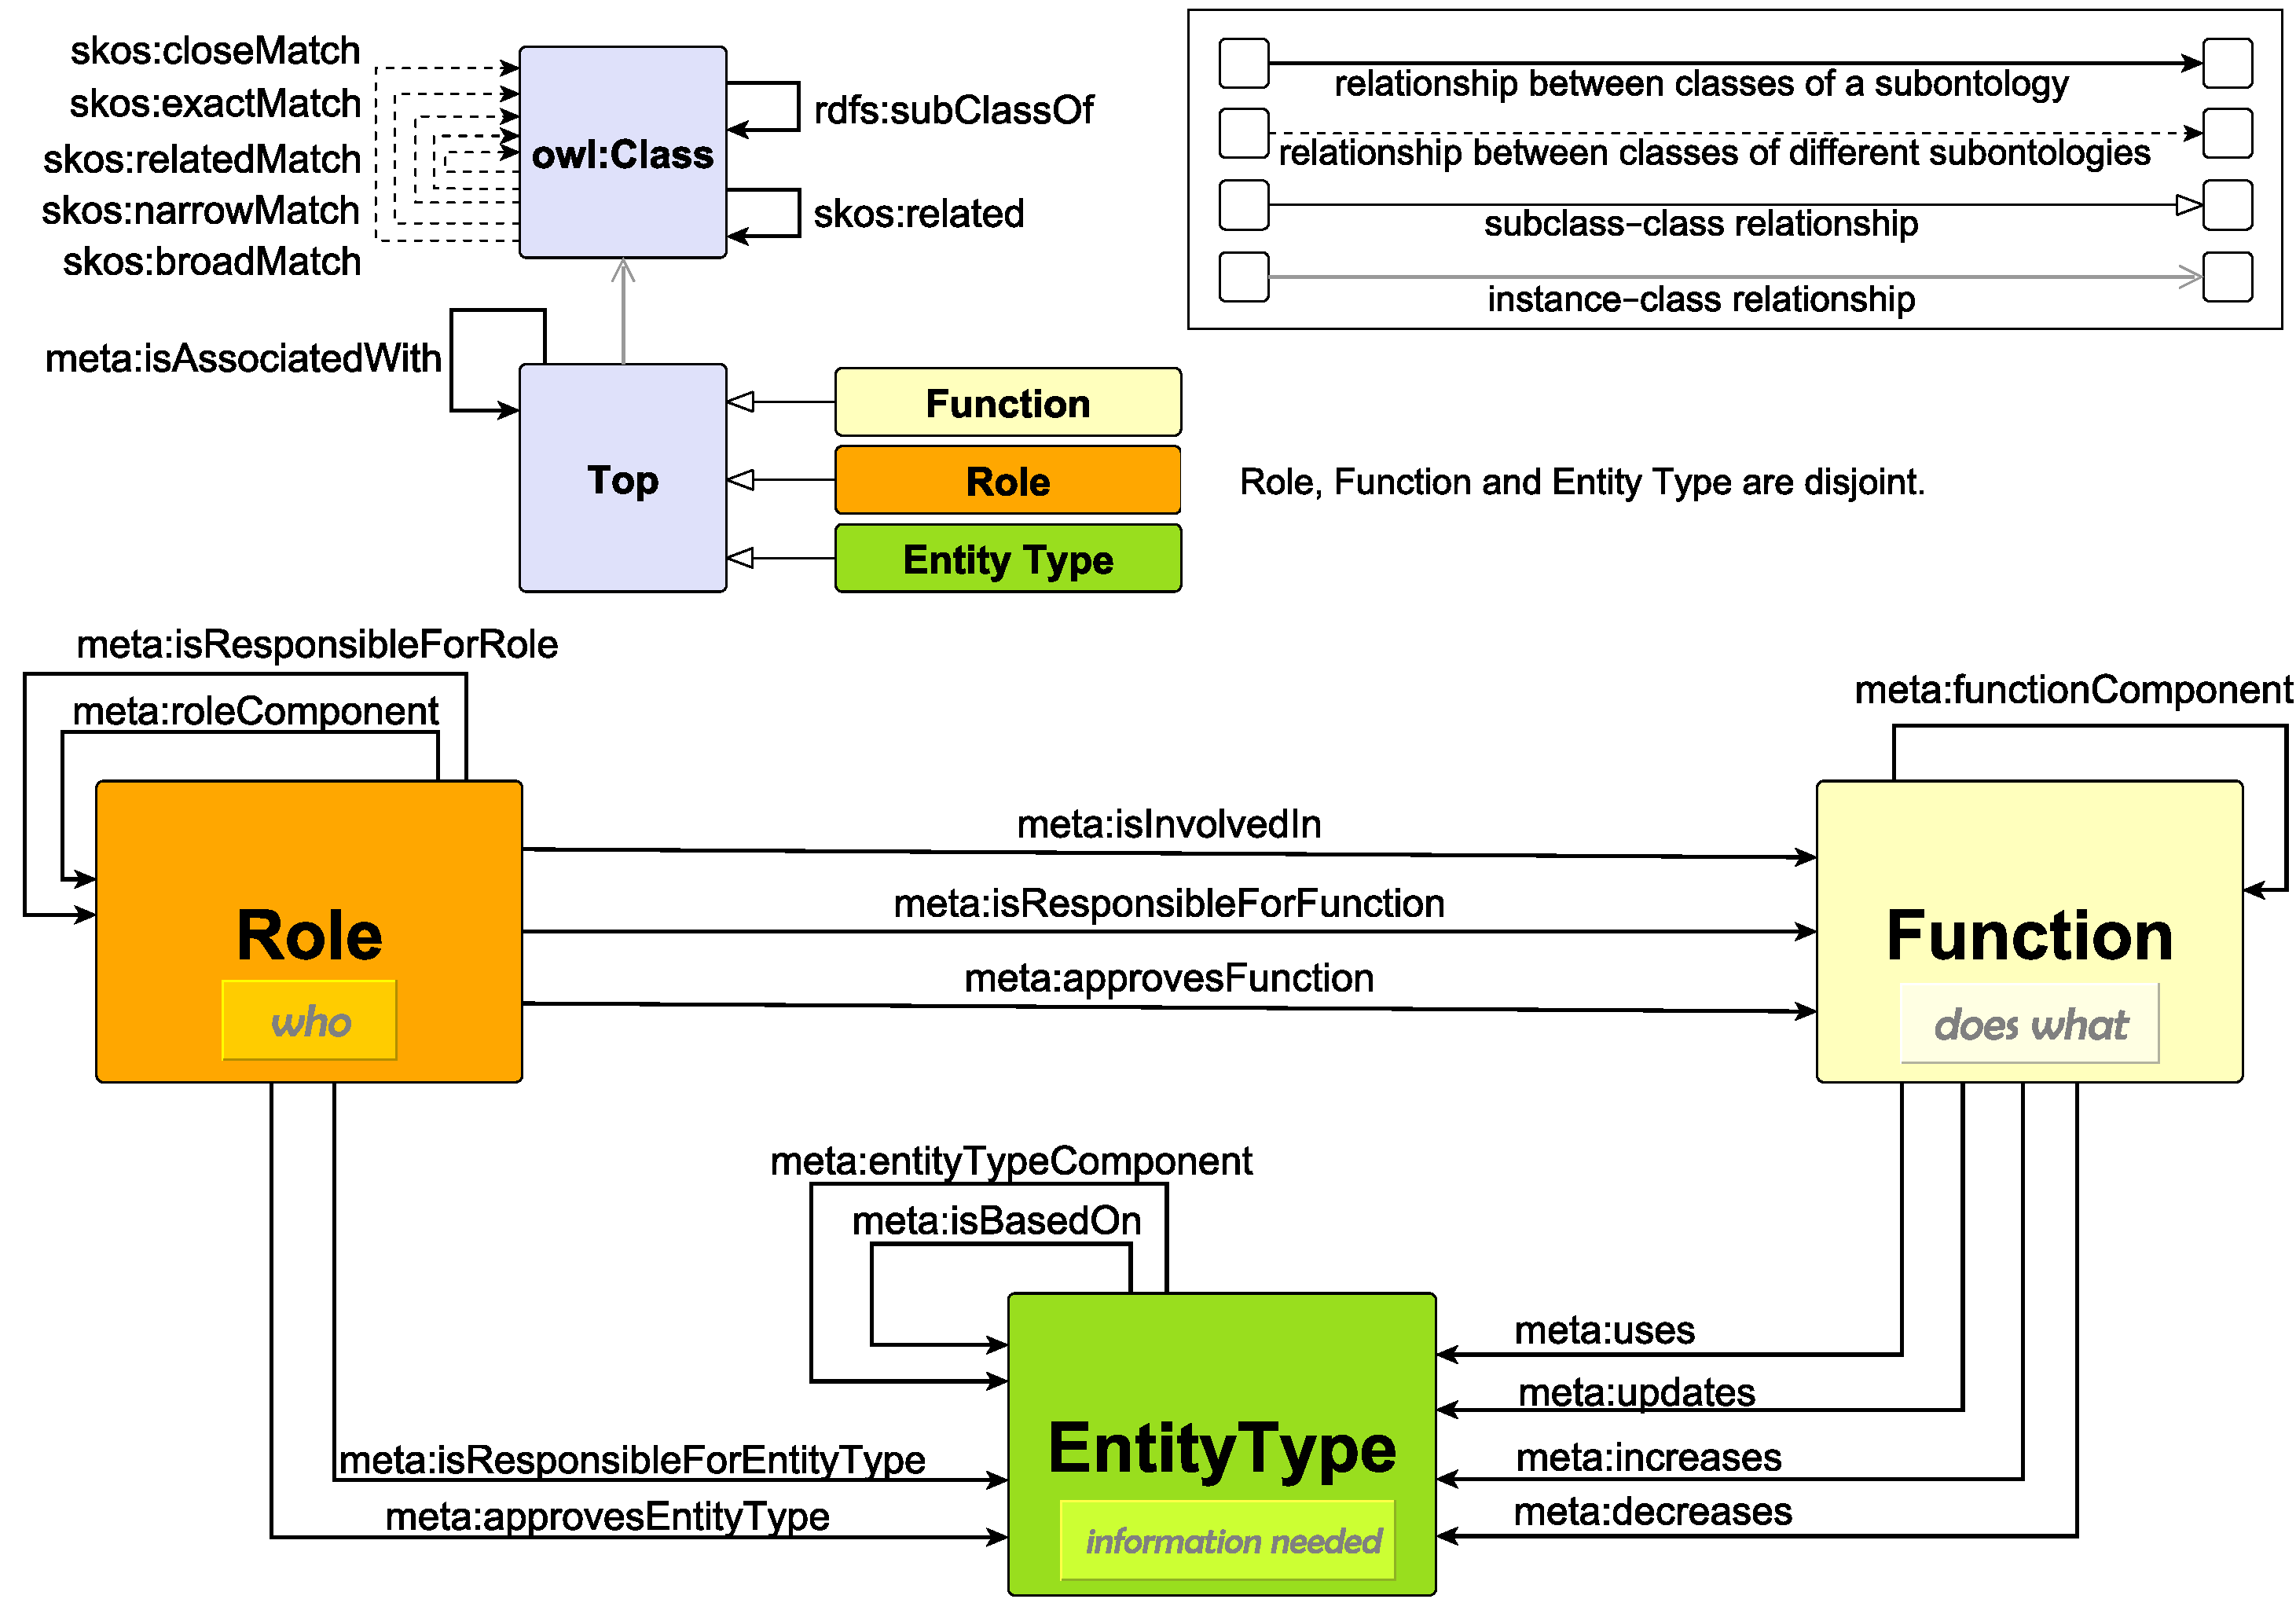
\includegraphics[width=0.8\textwidth]{img/metamodel9s.pdf}
\end{figure*}

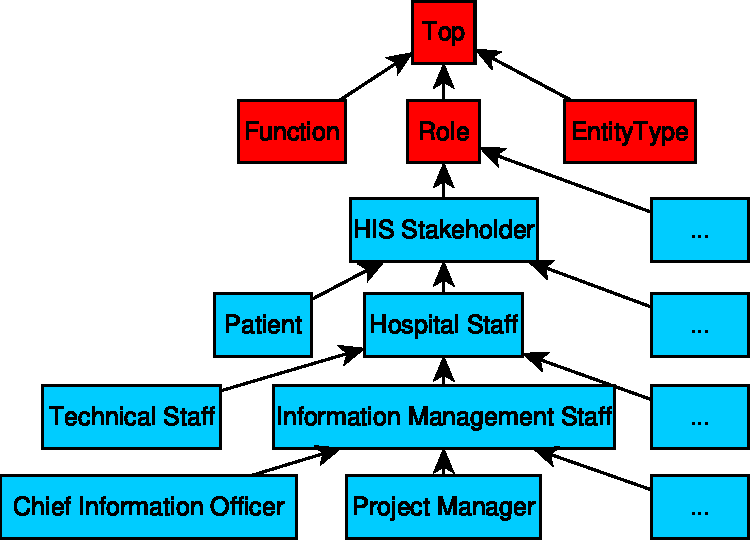
\includegraphics[width=\columnwidth]{img/hierarchy.pdf}
\begin{center}
\begin{tabular*}{\columnwidth}{ll}
\toprule
\textbf{Ontology}				&\textbf{Source}\\
\midrule
\url{http://www.snik.eu/ontology/meta}		&Meta Model\\
\url{http://www.snik.eu/ontology/bb}		&Textbook~\cite{bb}\\
\url{http://www.snik.eu/ontology/ob}		&Textbook~\cite{ob}\\
\url{http://www.snik.eu/ontology/he}		&Textbook~\cite{he}\\
\url{http://www.snik.eu/ontology/ciox}		&CIO Interview\\
\url{http://www.snik.eu/ontology/it4it}		&Standard~\cite{it4it}\\
\bottomrule
\end{tabular*}
\end{center}

\section{Sources}\label{sec:sources}
Three textbooks provide different views on the domain of Hospital Information Management:
\citet{bb} presents a broad view on \enquote{typical architectures of health information systems and their systematic strategic management}.
\citep{ob} concentrates on the \emph{tactical} management of information systems in general and on healthcare in particular.
The focus of tactical management lies on the planning and operation of projects.
\citet{he} explains information management beyond the scope of healthcare.
Other sources are interviews and standards.
%CIOX is based on an interview with the CIO of the Universitätsklinikum Leipzig.
%IT4IT is based on the IT4IT standard.\todo{Sebastian: Was über Standards und IT4IT schreiben}

\section{Data Model}\label{sec:architecture}
The initial structure of the meta model is defined in \citet{domaene}.
The \enquote{meta model} defines three basic disjunctive classes and their possible relations: Roles (who), Function (does what) and Entity Types (and which information is therefore needed).
A set of modular subontologies define subclasses of those three classes and their relations as described by a certain knowledge source about information management in hospitals:
The \textbf{Semantic Network of Information Management in Hospitals} (SNIK\footnote{Hospital means \enquote{Krankenhaus} in German.}) is a modular OWL 2 DL ontology.
%from different sources:% three textbooks, an interview and a standard.

\section{Data Set Description}\label{sec:dsd}
\begin{table*}
\caption{use of established vocabularies}
\label{tab:templates}
\begin{tabulary}{\textwidth}{lL}
\toprule
\textbf{Vocabulary}	&\textbf{Description}\\
\midrule
&\\
&\\
&\\
\bottomrule
\end{tabulary}
\end{table*}

The SNIK ontologies are available at \url{http://www.snik.eu/ontology/} under the Creative Commons Attribution-NonCommercial-ShareAlike 4.0 International license.

\section{Data Transformation Process}
\subsection{Interlinking}
%As shown in \cref{...}, we aligned our dataset to several others:
We manually aligned our dataset to HITO, the Health IT Ontology~\citep{hito}
We automatically aligned our dataset to:
- DBpedia~\citep{dbpedia}, as  
- 
\section{Lifecycle}\label{sec:application}

\begin{figure}[ht]
\caption{The SNIK lifecycle}
\label{fig:lifecycle}
\includegraphics[width=\columnwidth]{cycle.pdf}
\end{figure}

When we add a new textbook to SNIK, we identify all concepts that fit the meta model and their relations to other concepts.
Some project members are not proficient in RDF serializations, so we first fill out a meta model conforming spreadsheet template.
We then use Tarql\footnote{\url{https://github.com/cygri/tarql}} with a mapping configuration file\footnote{\url{https://github.com/IMISE/snik-csv2rdf}} to convert that spreadsheet to RDF.
Next, we refine the data in Protégé and upload it to a Virtuso SPARQL endpoint.

After the initial publish phase, we describe the repeating steps of the reuse phrase with the SNIK lifecycle in \Cref{fig:lifecycle}:
\begin{enumerate}
\item the Virtuoso SPARQL endpoint is used for querying and as data source for all our applications  
\item an instance of the OntoWiki~\citep{ontowiki} is used for punctual changes and additions by non-Semantic-Web-experts, supplemented by SPARUL for changes involving large numbers of classes 
\item LIMES~\citep{limes} generates interlink candidates between the different textbooks, which can be approved or rejected by the users
\item LodView\footnote{\url{https://lodview.it/}} lets the user browse among the classes of SNIK and view particular classes in detail
\item SNIK Graph, detailed in \Cref{sec:snik-graph}, supplements the RDF browser by visualizing the relationships between classes.
Users often discover incorrect modelling or possibilities for enhancement in SNIK graph.
\item SNIK quality is a web application that uses SPARQL queries to find problems of varying degree, such as violations of domain, range or naming conventions, subclass cycles or missing definitions.
\item Problems suggested by users and SNIK quality are verified, solved, and published on the SPARQL endpoint using SPARUL queries, at which point the circle begins anew.
\end{enumerate}

%After the initial extraction step, SNIK is published and users suggest problems or enhancements.%Besides issues of collaborative editing, this required a regular export and reupload, which delayed the effect of changes in SNIK to the user facing applications.
%- git repository (link): collaborative editing but protege can cause large diffs -> people who understand rdf enough to use text editor ttl/rdfxml 
%- use ontowiki: slow but user friendly, undo function,
%- SPARUL queries
The technical environment of those services is described in~\citet{sniktec}.
Selected applications are described in the following section.


\section{Data Quality}


\section{Applications}
SNIK was initially intended~\citep{domaene} both as  software to support hospital CIOs and to support teaching.
For the former goal, two applications were designed and implemented as prototypes~\citep{toreonto}: (1) the requirements engineering decision support system TOREOnto and (2) the knowledge exploration and navigation visualization CIONx.
Due to internal regulations, efforts to integrate them into the informational infrastructure of the Uniklinikum Leipzig were stopped.
Consequently, the other approaches are in the area of teaching support:

\subsection{SNIK Graph}\label{sec:snik-graph}
\todo{reference franziskas poster in both figures}
\todo{get a higher quality version of overview graphic}
\todo{reference \citet{visualizationoflargeontologies}}

\begin{figure}
\caption{SNIK Graph Overview. Source: \protect\citet{snikgraph}.}
\label{fig:snik-graph-overview}
\includegraphics[width=\columnwidth]{img/snik-graph.png}
\end{figure}

\begin{figure}
\caption{A teacher prepares a lecture on strategic HIS directing using the \enquote{Circle Star} function of SNIK Graph. Source: \protect\citet{snikgraph}.}
\label{fig:snik-graph-circle-star}
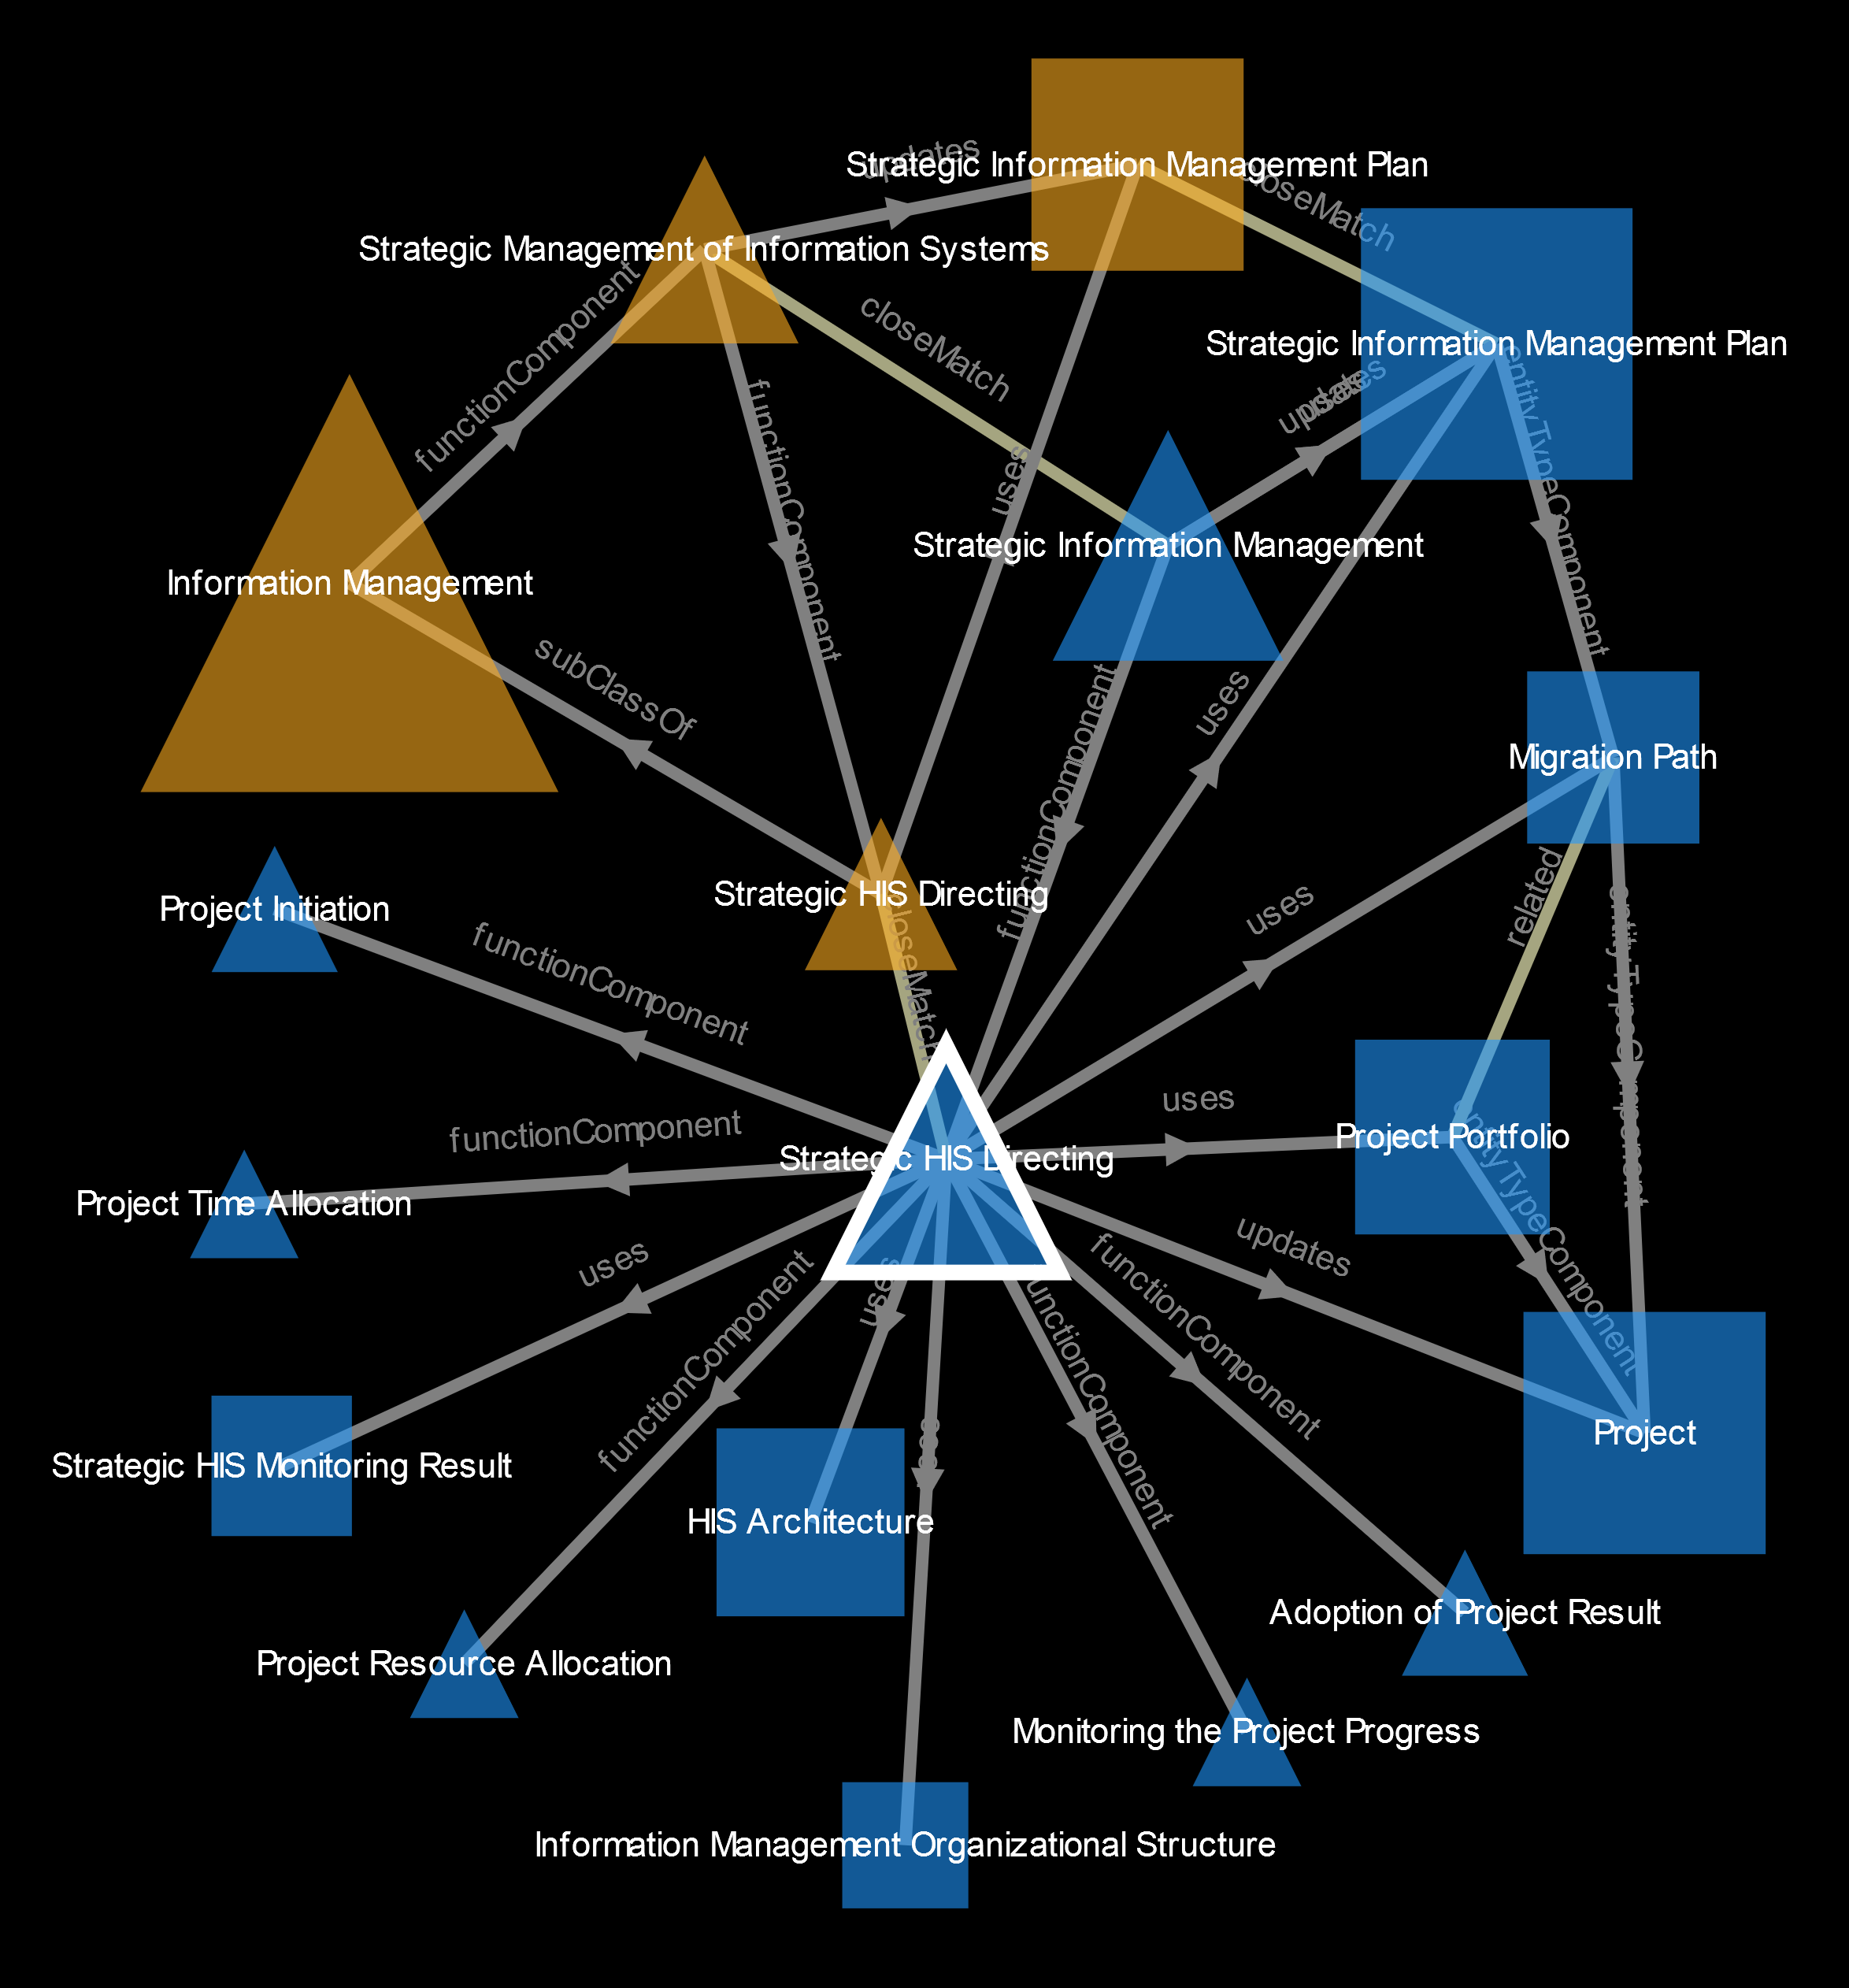
\includegraphics[width=\columnwidth]{img/snik-graph-circle-star.png}
\end{figure}

\begin{figure}
\caption{Students learn new concepts about HIS quality by linking them to concepts already learned.
A teacher asks a student to find out how the new concept \enquote{Quality of Data} is linked to the \enquote{Patient Identification Number}.
The student connects the two concepts by using the “spiderworm“ visualization and learns that a patient identification number is associated with object identity.
Object identity is a subclass of integrity of data.
Besides integrity of data, there are also 13 other criteria for quality of data.}
\label{fig:snik-graph-spiderworm}
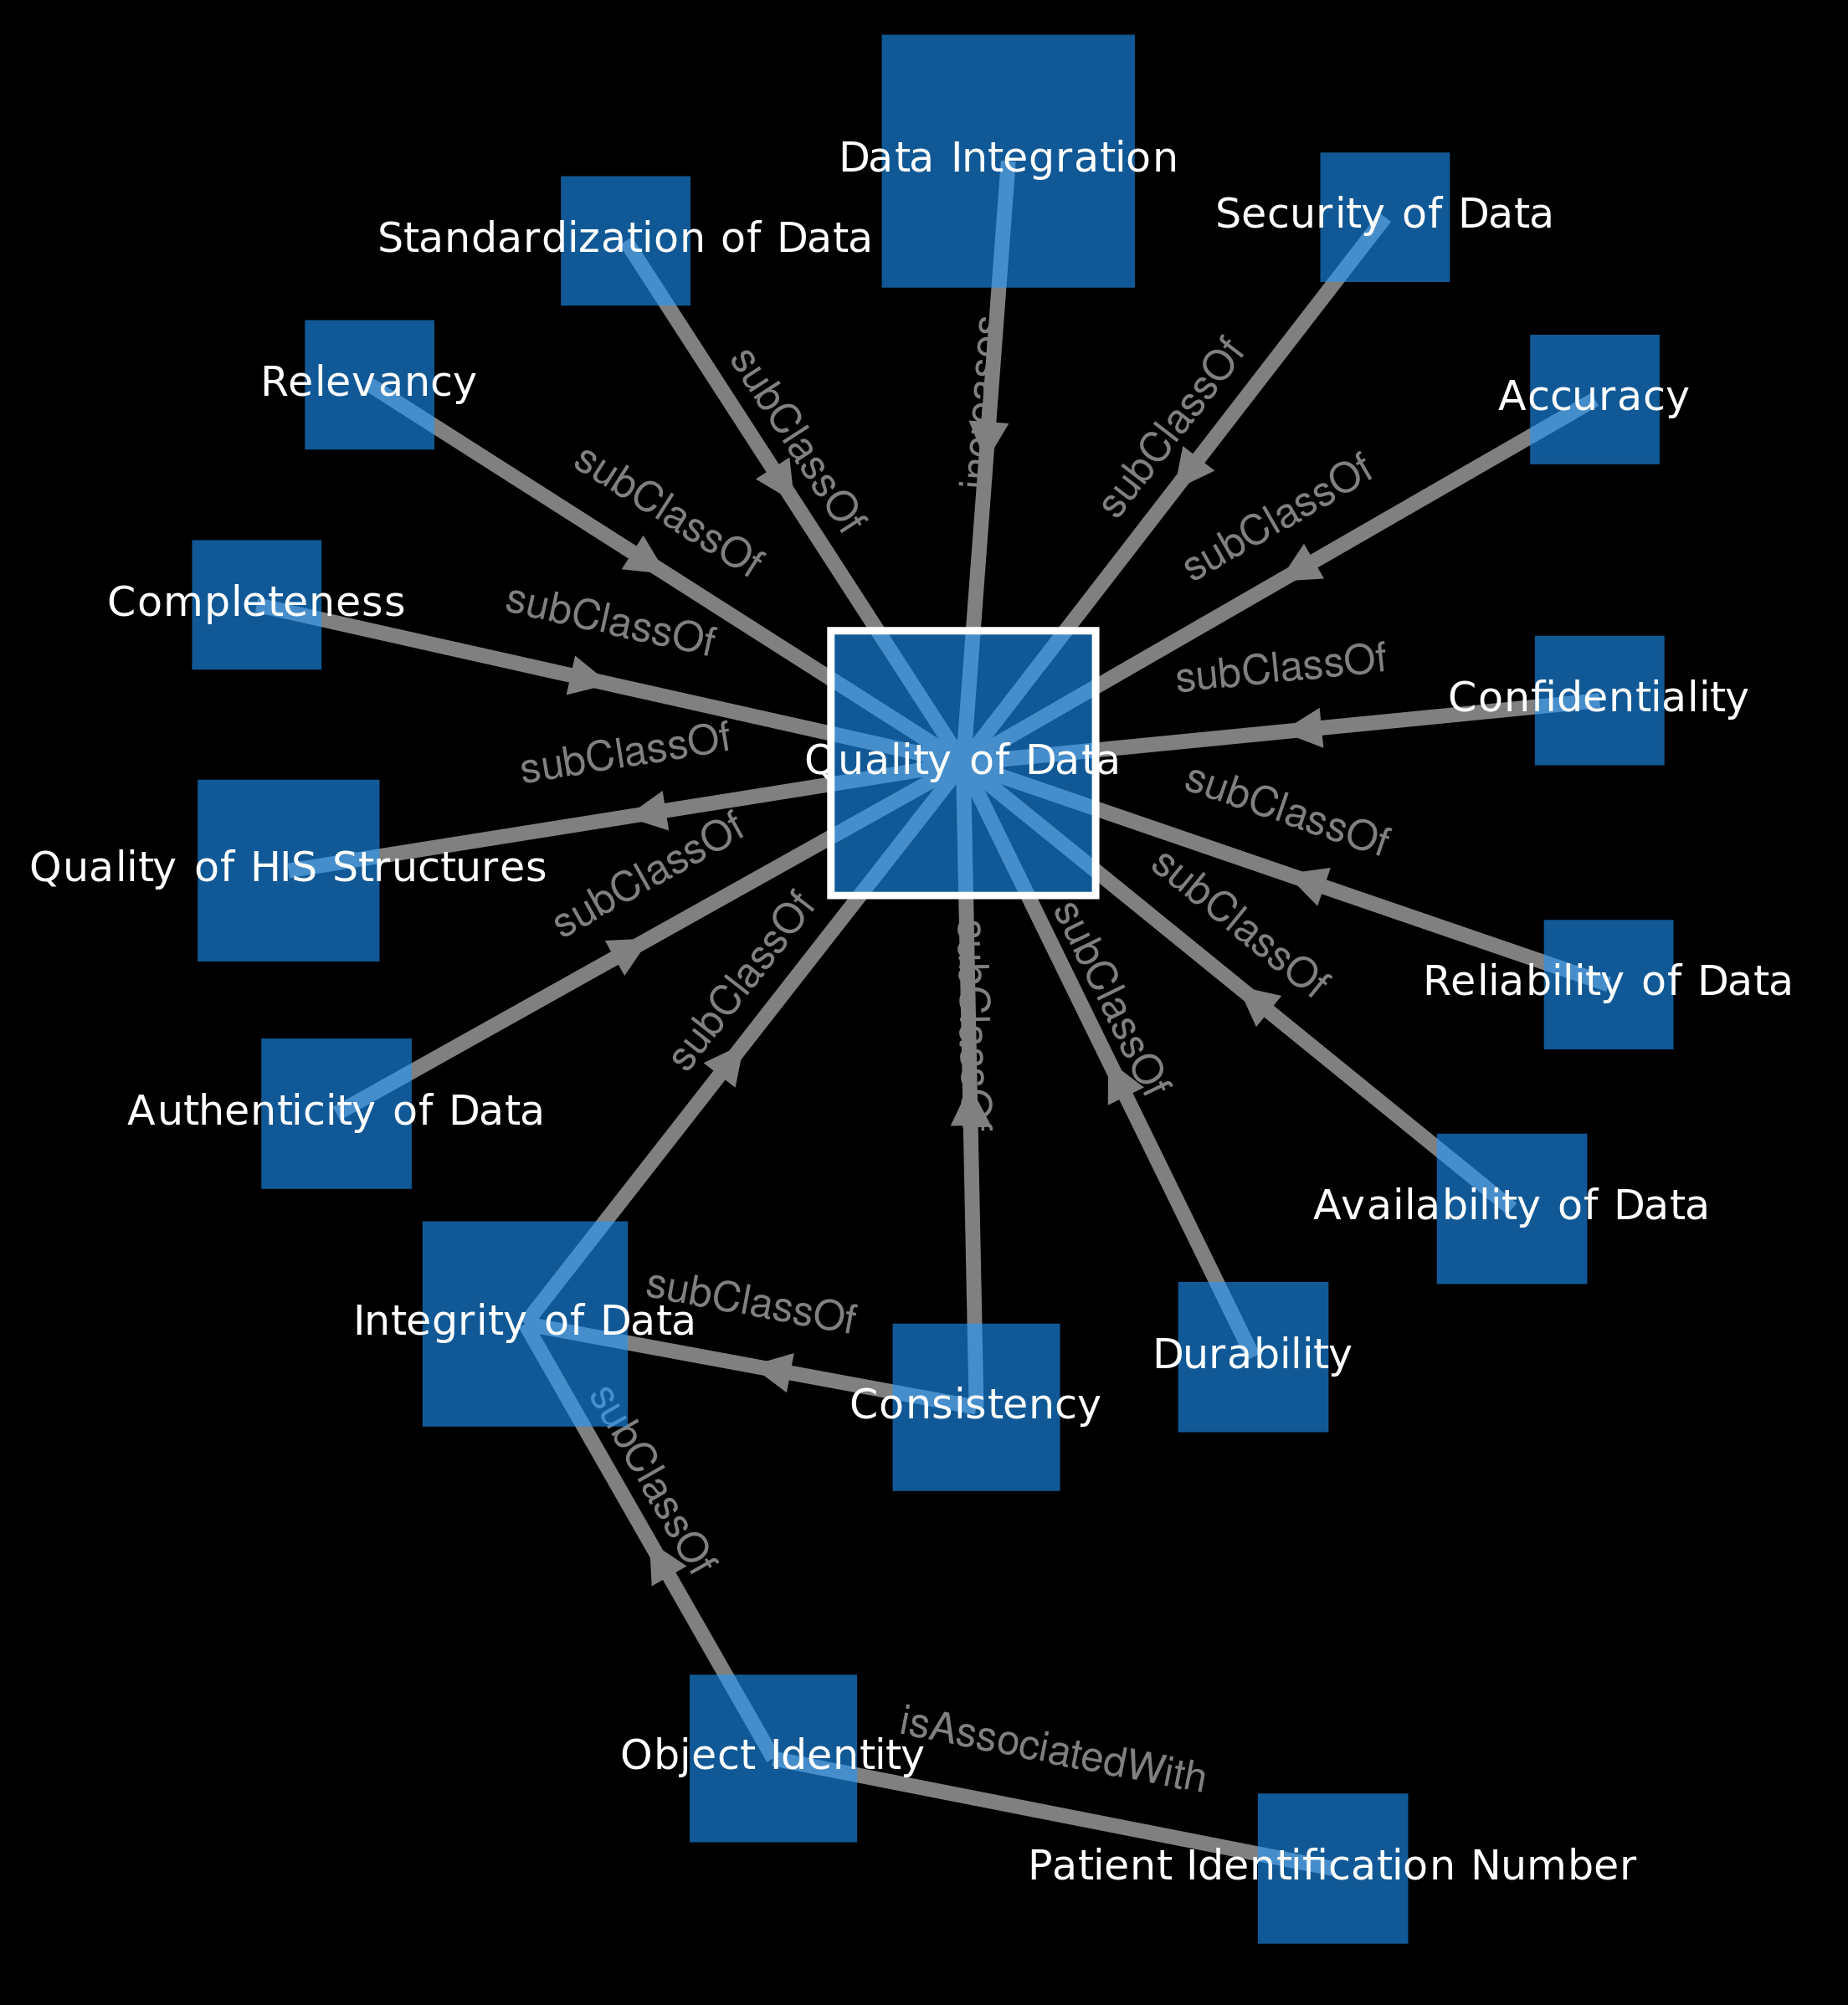
\includegraphics[width=\columnwidth]{img/snik-graph-spiderworm.png}
\end{figure}
\todo{FJ: In diesem Abschnitt fehlt die Diskussion, wie es durch die verschiedenen Zielgruppen bei Use Cases genutzt werden kann.}
SNIK Graph is a web application\footnote{\url{http://www.snik.eu/graph}} that transforms the classes and triples of SNIK to nodes and edges of a graph.
The graph is visualized using the Cytoscape.js~\citep{cytoscape} library with the force-directed Euler layout, see~\cref{fig:snik-graph-overview}.
With several thousand classes, specific parts of SNIK can be hard to discern.
Thus, there are several options to view subgraphs of SNIK, for example to show only a specific chapter of a book to prepare a lecture about a specific topic.
Users can also search for and restrict the view to a single class and then show the neighbourhood of that class (see \cref{fig:snik-graph-circle-star}) and subsequently the neighbourhood of selected neighbours of the previous step.
SNIK Graph can also calculate the shortest path to between classes.
We also tried to automatically find the most interesting path but this was not successfull as it is subjective and the depends on the goal of the user.
Path and neighourhood operations are joined in the \enquote{spider worm} (see \cref{fig:snik-graph-spiderworm}), which consists of the shortest path between a start node and an end node together with the end node’s neighbourhood, illustrate the context of a concept.

\subsection{Quiz}
The DBpedia-powered Clover Quiz~\citep{cloverquiz} shows that ontologies can be used to automatically generate multiple-choice questions.
We apply this approach to SNIK and generate 1231 English questions using the templates described in \cref{tab:templates}.
It was used by students from the Universities of Amsterdam, Heidelberg and Leipzig during the international Frank van Swieten lectures in 2019.
To provide difficult wrong answers, the so called \emph{distractors}, we use direct neighbours of the classes that represent the correct answers.
Due to the limited nesting capabilties of SPARQL, which does not support loops but only subqueries that cannot access variables declared outside their scope, querying for distinct sets of 4 neighbours, where exactly one was connected over a certain property to a certain object, was not possible with our Virtuoso SPARQL endpoint initially.
We circumvented the timeout by calculating the neighbour-relation as a first step and uploading it to the endpoint.

%SNIK Quiz is freely available as an open source web application.
Because SNIK only contains the knowledge that the source textbooks describe, it does not contain the complete domain of Hospital Information Management.
As such, negative questions are problematic, as the given relationship could hold in the real world but not be described in the textbook source of the class.
The same problem concerns the distractors of positive questions.
So this problem cannot be avoided.
However, this is one of the reasons that we don't ask count questions like \enquote{How many functions is the CIO responsible for?}, which don't help much for learning anyways. % improve writing
Relationships could also hold implicitly through the subclass hierarchy.
For example, \aurl{bb}{ChiefInformationOfficer} is a subclass of \aurl{bb}{InformationManagementStaff}, which is responsible for \aurl{bb}{OperationalInformationManagement}.
It is unclear, whether the CIO is also responsible for operational information management.
In the future, we will add more question types 

\begin{table*}
\caption{Templates}
\label{tab:templates}
\begin{tabulary}{\textwidth}{lL}
\toprule
\textbf{Template}	&\textbf{Description}\\
\midrule
Definition		&Ask for the class that fits the given textbook definition.\\
Example			&What is defined as \enquote{Examination of in and out patients in radiological department}?\\
Distractors		&Labels of other classes (that have a path of length 2 or less to the correct class.)\\
\midrule
Subject			&Ask for the class that is related via a given relation to a given object.\\
Example			&Who is \emph{involved in} a \emph{healthcare network}?\\
Distractors		&Labels of other classes (of the same type) that \emph{are not} related via the same relation to the same object.\\
\bottomrule
\end{tabulary}
\end{table*}



%The technical environment of SNIK is characterized in previous work [11].
\section{Discussion}
SNIK is based on the meta model from Figure \todo{reference}.
Thus, SNIK can be considered as an archetype for ontologies describing for a given domain (here \enquote{HIS management}), what functions a certain role has to carry out and what information a person of this role needs and what information she/he provides while carrying out the functions.
This may be used for domains like the medical department of a hospital as well.\todo{FJ: Ich glaube, das müsste man ausführlicher erklären, das würde ich eher ans Ende der Diskussion nehmen.}
This would be valuable knowledge, for instance as basis for systems analysis projects [1].
Different user groups can use the interfaces of SNIK that are most suitable to them.
For example, the IT management of a hospital can use SNIK as a vocabulary to integrate data from different formats that result from application components from different vendors.
Using the SPARQL1 query language, experts can also integrate applications with the SNIK ontology.
 Experts can also use the SPARQL query editor to answer specific questions, see Table 2.
Students and teachers, on the other hand, benefit more from SNIK Graph, which intuitively presents knowledge without the need for technical skills.

Figure 4– A \enquote{Spider Worm} between the classes \enquote{Change Management} and \enquote{HIS Quality} in the SNIK Graph visualization web application.
The content of SNIK is taken from textbooks which are protected by property rights of publishing houses or taken from an interview with a CIO holding property rights as well.
Making the SNIK ontology openly available may therefore conflict with these property rights.
In case of SNIK, we appreciate the approvals of the publishing houses Springer, de Gruyter and Schattauer and of the CIO.
In general, missing approvals may prevent the creation of such open ontologies and thus the provision of textbook content as open knowledge.
The approvals for SNIK were possible because for each class and relation being part of SNIK there is a clear indication of its source (see code \enquote{bb} and chapter information in Table 1).
In future work we will use these indications for establishing hyperlinks into the sources such that users of SNIK may use SNIK as a smart index for retrieving more detailed knowledge and supporting illustrations from the original textbooks – if digitally available.
We are convinced that this way an ontology like SNIK is not a competitor of textbooks but a smart guide for using a textbook.
Thus, it might be attractive for publishing houses.

\todo{verweis auf existierende papers}
\todo{benutzung durch braunschweig}
\todo{benutzung durch amsterdam}

\section{Conclusions}
We showed that knowledge on the management of information systems in medicine and health care is made publicly available using open standards over several interfaces with different compromises between expressivity and accessibility.
It can be combined with other knowledge in biomedical and health informatics and in other disciplines.

\section{Future Work}
\todo{Connection with HITO}
We plan to extend the text-based interlinks with semantic-similarity-based ontology matching [5] to find more correspondencies between the textbooks.
This will enable users to switch to another textbook when a certain concept is explained there in more detail.
The SNIK toolset, SNIK Graph in particular, is under permanent improvement.
For instance, we are considering alternatives to the shortest path that are the most preferred by different audiences and whether those paths can be (semi-)automatically generated using suitable node or edge weight functions.
We are also investigating candidates for additional subontologies and as interlink targets.

\section{Acknowledgments}
This work is supported by the DFG (German Research Foundation) under the Projects SNIK, grant no. 1605/7-1 and 1387/8-1, as well as HITO, grant no. WI 1605/11-1 and I3726-N31.
%We thank the publishers ... and ... for granting us permission to publish the subontologies based on the textbooks \citet{bb,ob,he} under an open license.
%\nocite{*} 
\todo{FJ: Hmmm, ziemlich selbstreferenziell. Brauchen wir da wirklich so viele Publikationen von uns? Welche anderen könnte man noch einbringen? Ich schaue auch mal, was mir so über den Weg läuft.}
\bibliographystyle{ios1}
\bibliography{paper,snik}
\section{Notes to Reviewers}
This paper includes and extends text and figures from:
\citet{snikgraph}

\end{document}
